\documentclass{beamer}
\usepackage[utf8]{inputenc}
\usetheme{Singapore}
\usecolortheme{default}
\usepackage{graphicx}
\beamertemplatenavigationsymbolsempty


\title[Genetic algorithm for QSVM] 
{Genetic algorithm for Quantum Support Vector Machines}



\author[Lorenzo Tasca]
{Lorenzo Tasca}
 

\date[25/11/2024] 
{25 Novembre 2024}

\logo{
\includegraphics[height=1cm]{images/logo.png}}

\begin{document}

\frame{\titlepage}

\begin{frame}
\frametitle{Quantum Machine Learning}
\centering
\begin{figure}
      
\includegraphics[width=1.1\textwidth]{images/1.png}
     \end{figure}
\end{frame}



\begin{frame}
  \frametitle{Support Vector Machine}
    \begin{itemize}
      \item     La Support Vector Machine è un algoritmo supervisionato di classificazione binaria. 
    \end{itemize}
      \begin{figure}
            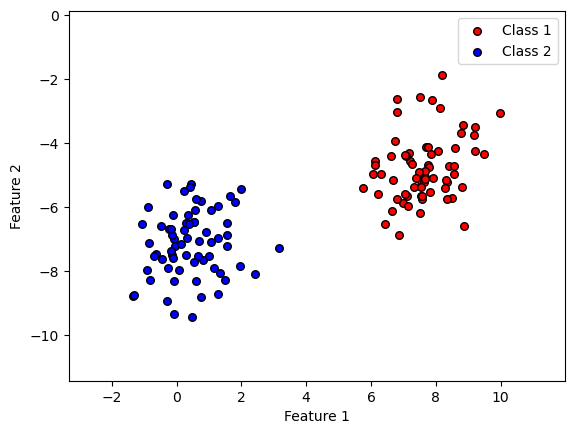
\includegraphics[width=0.7\textwidth]{images/classicaldata.png}
       \end{figure}
  \end{frame}



  \begin{frame}
    \frametitle{Support Vector Machine}
      \begin{itemize}
        \item L'algoritmo trova il massimo margine separatore tra le classi. 
      \end{itemize}
        \begin{figure}
              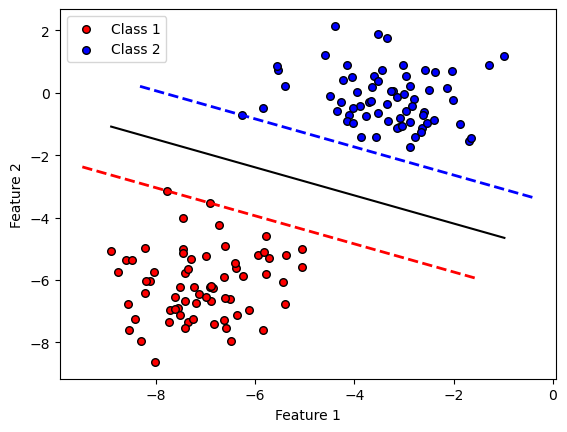
\includegraphics[width=0.7\textwidth]{images/classicalsvm.png}
         \end{figure}
    \end{frame}


    \begin{frame}
      \frametitle{Support Vector Machine}
        \begin{itemize}
          \item Per farlo utilizza solo i prodotti scalari tra i dati $\langle \mathbf{x}_i, \mathbf{x}_j\rangle$.  
        \end{itemize}
          \begin{figure}
                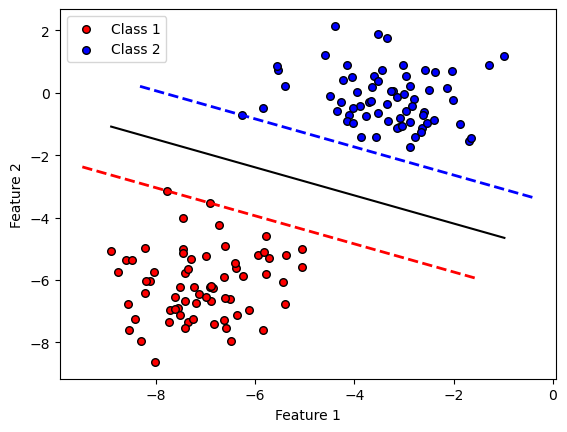
\includegraphics[width=0.7\textwidth]{images/classicalsvm.png}
           \end{figure}
      \end{frame}


\begin{frame}
  \frametitle{Kernel Support Vector Machine}
  
  \begin{itemize}
    \item Nel caso in cui i dati non siano linearmente separabili?
  \end{itemize}
     
        \begin{figure}
          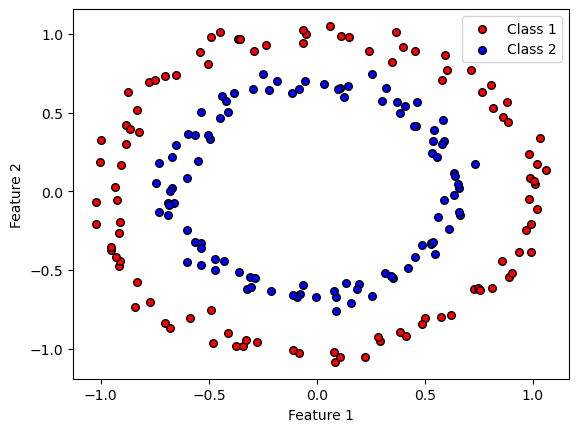
\includegraphics[width=0.7\textwidth]{images/circles.png}
        \end{figure}
        
\end{frame}

\begin{frame}
  \frametitle{Kernel Support Vector Machine}
  
  \begin{itemize}
    \item È possibile applicare una feature map $\phi(\mathbf{x})$.
  \end{itemize}
     
        \begin{figure}
          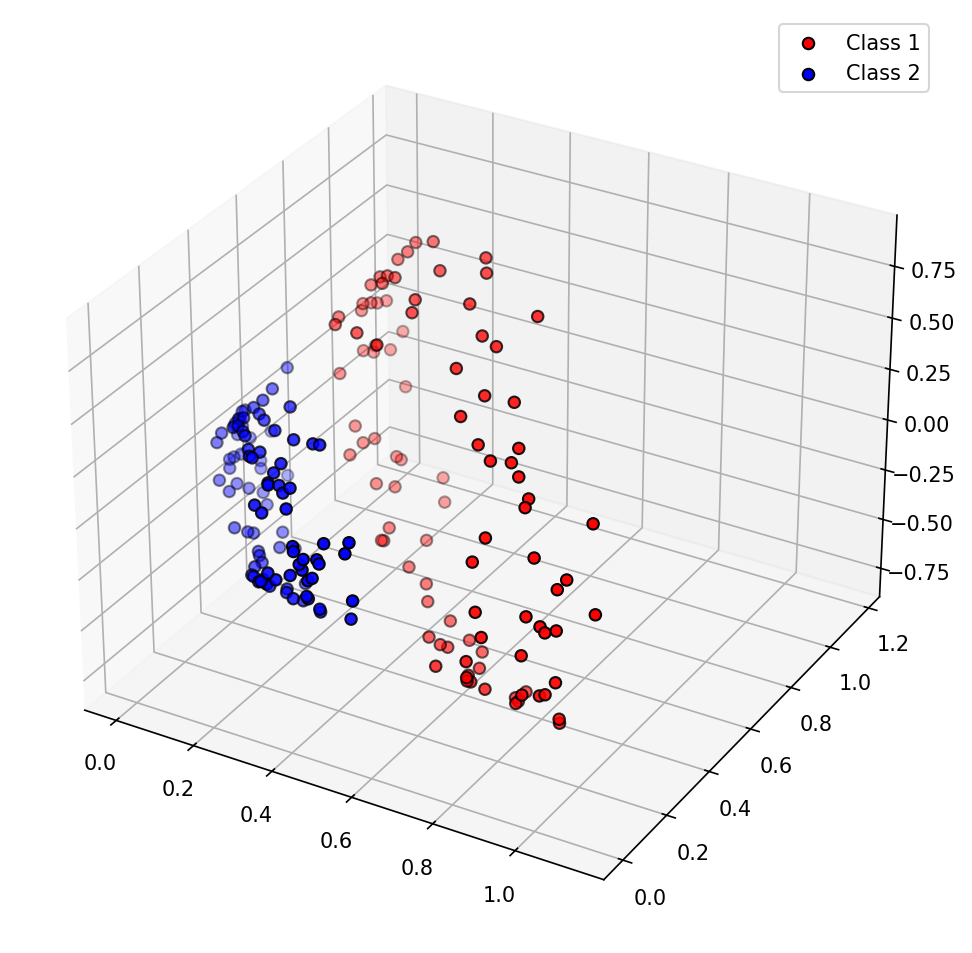
\includegraphics[width=0.6\textwidth]{images/circles3d.png}
        \end{figure}
        
\end{frame}

\begin{frame}
  \frametitle{Kernel Support Vector Machine}
  
  \begin{itemize}
    \item L'algoritmo è interessato solo a $K_{ij}=\langle \phi(\mathbf{x}_i), \phi(\mathbf{x}_j) \rangle$.

  \end{itemize}
     
        \begin{figure}
          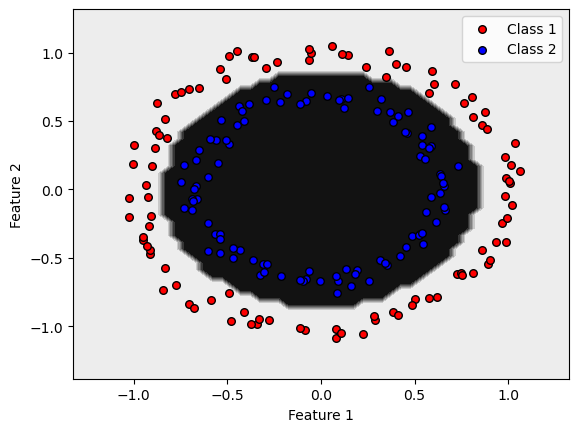
\includegraphics[width=0.7\textwidth]{images/separatedcircle.png}
        \end{figure}
        
\end{frame}








\begin{frame}

  \frametitle{Quantum Support Vector Machine}
  
  \begin{columns}
    \column{0.5\textwidth}
  
    \begin{itemize}
      \item<1-> La feature map diventa un circuito quantistico parametrizzato. \\\,
          \item<2-> $|\phi(\mathbf{x})\rangle=U(\mathbf{x})|0\rangle^{\otimes n}$.\\\,
          \item<3->  $K_{ij}=\langle \phi(\mathbf{x}_i)| \phi(\mathbf{x}_j) \rangle.$
          \end{itemize}
    
    \column{0.5\textwidth}
    \only{\begin{figure}
          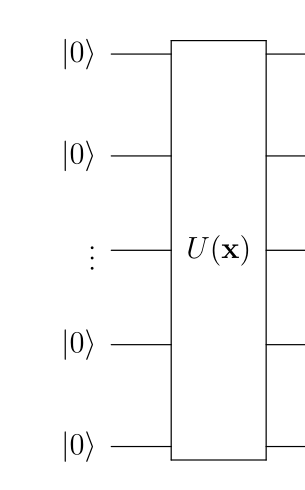
\includegraphics[width=0.7\textwidth]{images/Pasted image.png}
     \end{figure}}<1>
     \only{\begin{figure}
      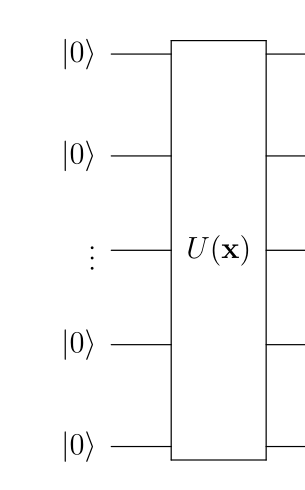
\includegraphics[width=0.7\textwidth]{images/Pasted image.png}
 \end{figure}}<2>
     \only{\begin{figure}
      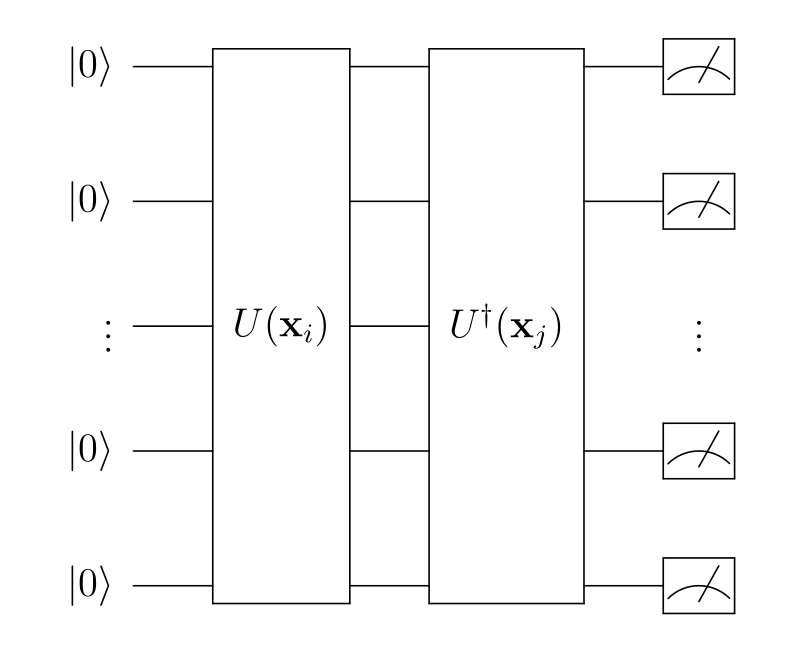
\includegraphics[width=\textwidth]{images/Pasted image (2).png}
 \end{figure}}<3>


    
    \end{columns}

\end{frame}


\begin{frame}
  \frametitle{Quantum Kernels}
  
  \begin{itemize}
    \item Un esempio possibile: la ZZ Feature Map. \\\,
  \end{itemize}
     
        \begin{figure}
          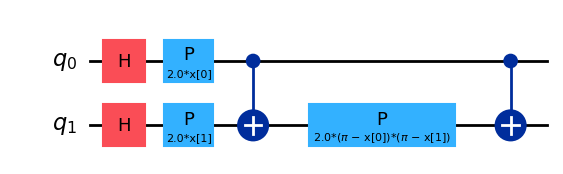
\includegraphics[width=\textwidth]{images/ZZ.png}
        \end{figure}
        
\end{frame}


\begin{frame}
  \frametitle{Quantum Kernels}
  
  \begin{itemize}
    \item Ottime performance su dataset complessi. 
  \end{itemize}
        \begin{figure}
          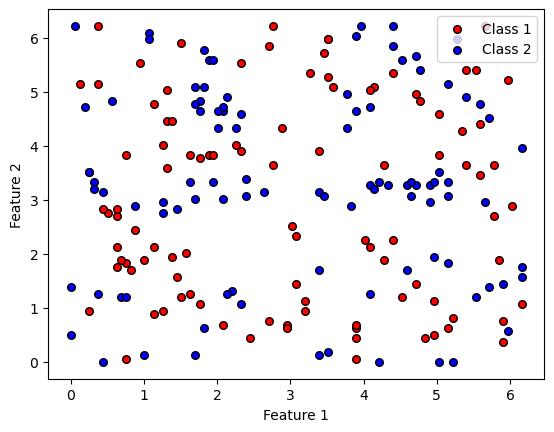
\includegraphics[width=0.7\textwidth]{images/adhoc.png}
        \end{figure}
        
\end{frame}

\begin{frame}
  \frametitle{Quantum Kernels}
  
  \begin{itemize}
    \item Ottime performance su dataset complessi.  
  \end{itemize}
        \begin{figure}
          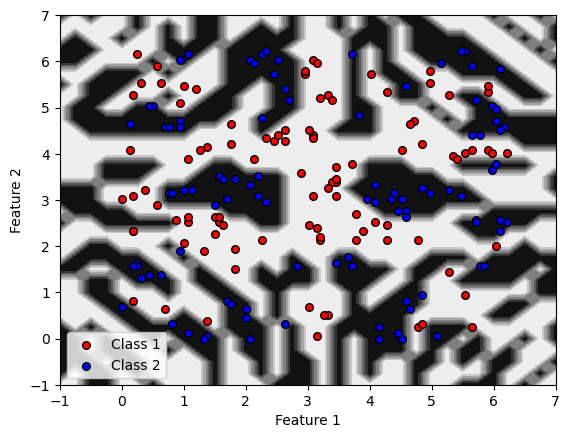
\includegraphics[width=0.7\textwidth]{images/adhoczz.png}
        \end{figure}
        
\end{frame}


\begin{frame}
  \frametitle{Quantum Kernels}
  \begin{itemize}
    \item I metodi classici falliscono.  
  \end{itemize}
        \begin{figure}
          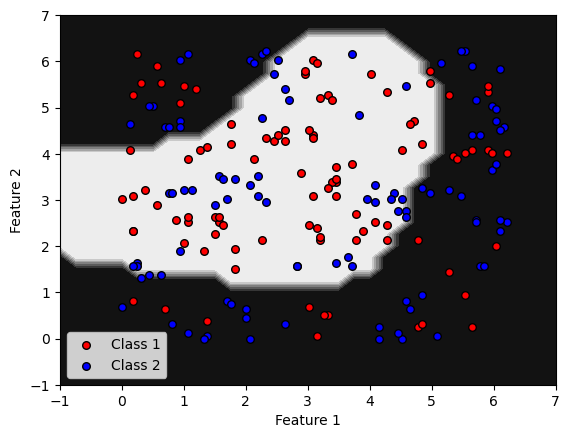
\includegraphics[width=0.7\textwidth]{images/adhocrbf.png}
        \end{figure}
        
\end{frame}


\begin{frame}
  \frametitle{Scelta del Quantum Kernel}
  \begin{itemize}
    \item La scelta del kernel risulta spesso problematica. 
  \end{itemize}
        \begin{figure}
          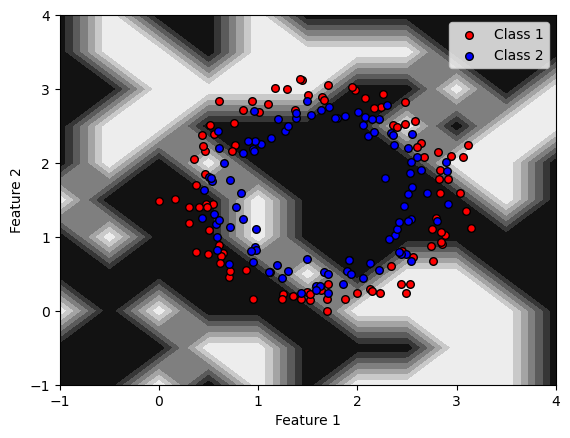
\includegraphics[width=0.7\textwidth]{images/failcircle.png}
        \end{figure}
\end{frame}

\begin{frame}
  \frametitle{Scelta del Quantum Kernel}
  \begin{itemize}
    \item Manca una guida per effettuare la scelta.
  \end{itemize}
        \begin{figure}
          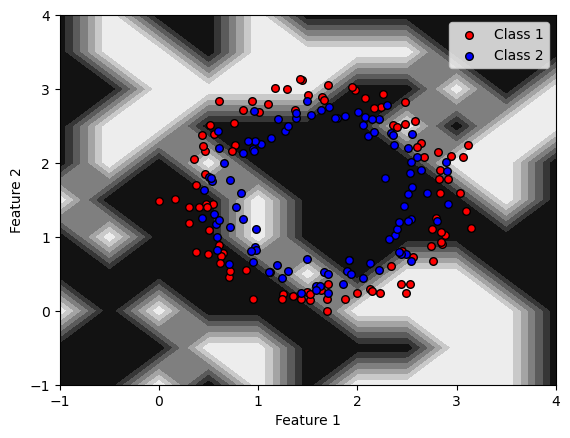
\includegraphics[width=0.7\textwidth]{images/failcircle.png}
        \end{figure}
\end{frame}



\begin{frame}
  \frametitle{Algoritmo genetico}
  \begin{itemize}
    \item Un algoritmo genetico può scegliere la miglior feature map.\\\,
  \end{itemize}

  \begin{figure}
    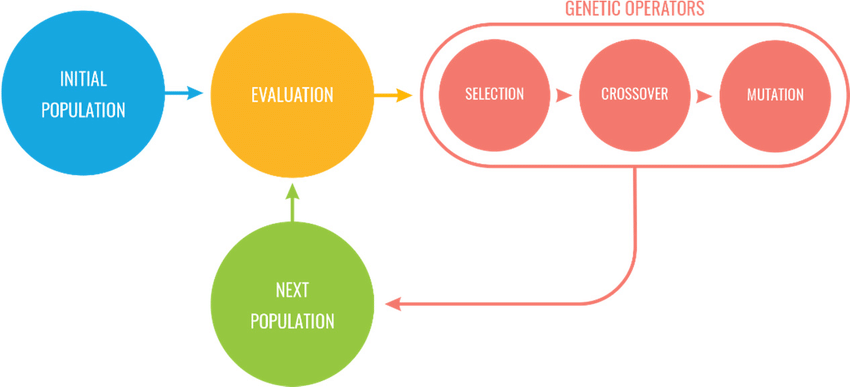
\includegraphics[width=\textwidth]{images/genetic.png}
  \end{figure} 
\end{frame}


\begin{frame}
  \frametitle{Algoritmo genetico}
  \begin{itemize}
    \item Gli individui sono formati da gate scelti da un set completo.\\\,
  \end{itemize}
  \begin{figure}
    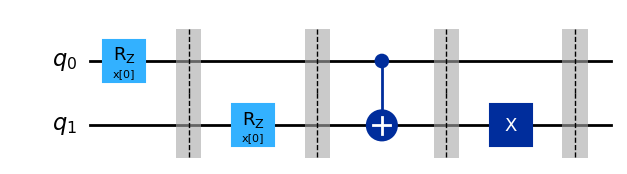
\includegraphics[width=\textwidth]{images/fenotip.png}
  \end{figure} 
\end{frame}

\begin{frame}
  \frametitle{Algoritmo genetico}
  \begin{itemize}
    \item La fitness di un individuo si calcola a partire dalla sua accuratezza.
  \end{itemize}

  \begin{figure}
    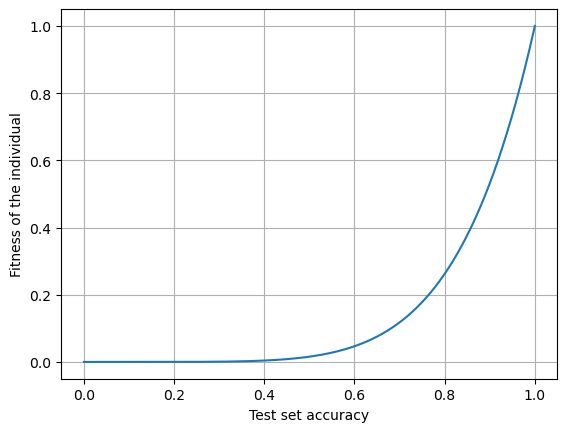
\includegraphics[width=0.7\textwidth]{images/sigmoid.png}
  \end{figure} 
\end{frame}

\begin{frame}
  \frametitle{Algoritmo genetico}
  \begin{itemize}
    \item La prima generazione è generata randomicamente. 
  \end{itemize}

  \begin{figure}
    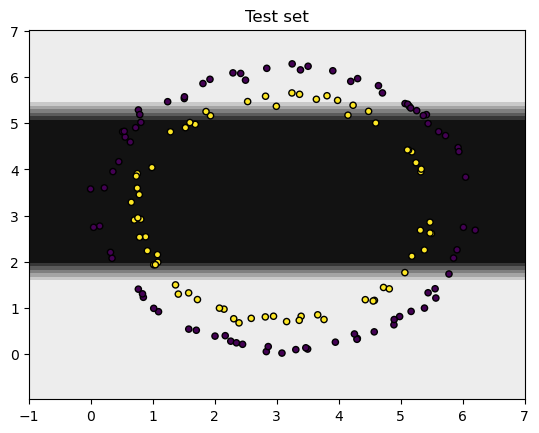
\includegraphics[width=0.7\textwidth]{images/badresult.png}
  \end{figure} 
\end{frame}

\begin{frame}
  \frametitle{Algoritmo genetico}
  \begin{itemize}
    \item Gli individui sono passati alla seguente generazione con il crossover.
    \vspace{0.5cm}

  \centering \textit{Parent individuals}    \,\,\,\,\,\,\,
  \end{itemize}
  \begin{minipage}{0.5\textwidth}
    \centering
    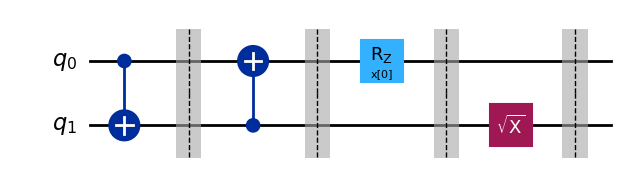
\includegraphics[width=\textwidth]{images/parent1.png}
\end{minipage}%
\begin{minipage}{0.5\textwidth}
    \centering
    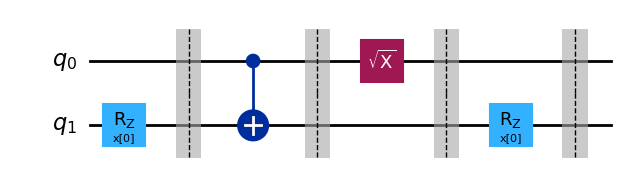
\includegraphics[width=\textwidth]{images/parent2.png}
\end{minipage}

\vspace{0.5cm}
\centering \textit{Child individuals}
\begin{minipage}{0.5\textwidth}
    \centering
    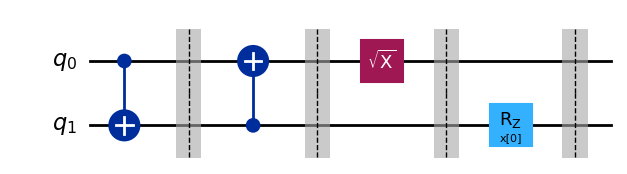
\includegraphics[width=\textwidth]{images/child1.png}
\end{minipage}%
\begin{minipage}{0.5\textwidth}
    \centering
    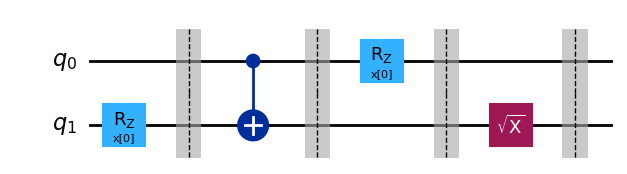
\includegraphics[width=\textwidth]{images/child2.png}
\end{minipage}

\end{frame}


\begin{frame}
  \frametitle{Algoritmo genetico}
  \begin{itemize}
    \item Inoltre subiscono una mutazione casuale.  
  \end{itemize}

  \begin{figure}
    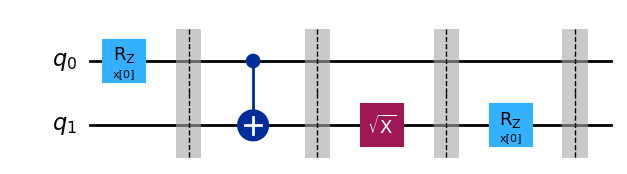
\includegraphics[width=0.9\textwidth]{images/nonmutated.png}
  \end{figure} 
  \begin{figure}
    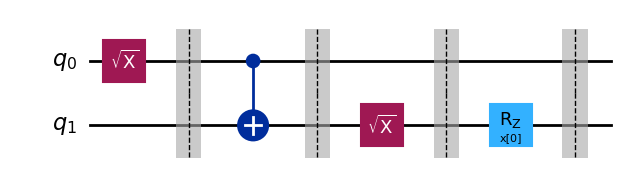
\includegraphics[width=0.9\textwidth]{images/mutated.png}
  \end{figure} 
\end{frame}

\begin{frame}
  \frametitle{Algoritmo genetico}
  \begin{itemize}
    \item Con l'andare delle generazioni aumenta l'accuratezza media.  
  \end{itemize}

  \begin{figure}
    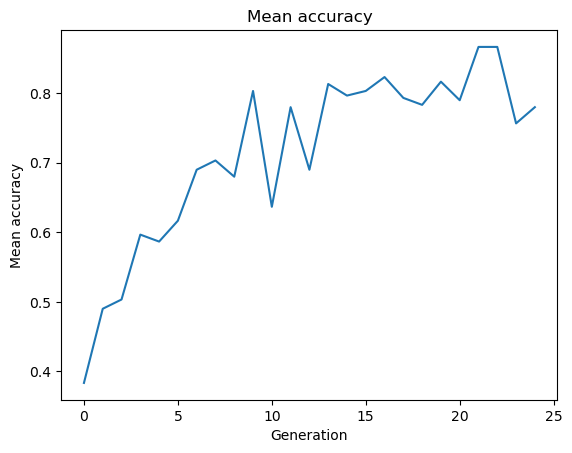
\includegraphics[width=0.7\textwidth]{images/meanaccuracy.png}
  \end{figure} 

\end{frame}










\end{document}